\section{Models}
To represent the real world using equations, we first need to define a model. A model is a \textbf{mathematical approximation} of
the real world, which allows describing events and phenomena using parametric representations. The parameters of the model
can be used for processing purposes.

\subsection{Pinhole Camera Model}
The first model we will discuss is the \textbf{pinhole camera model}, which relates to how a camera captures an image.
It assumes that an object in the real world emits light rays that pass through a small hole (the pinhole) and project onto an image plane.
\begin{figure}[H]
    \centering
    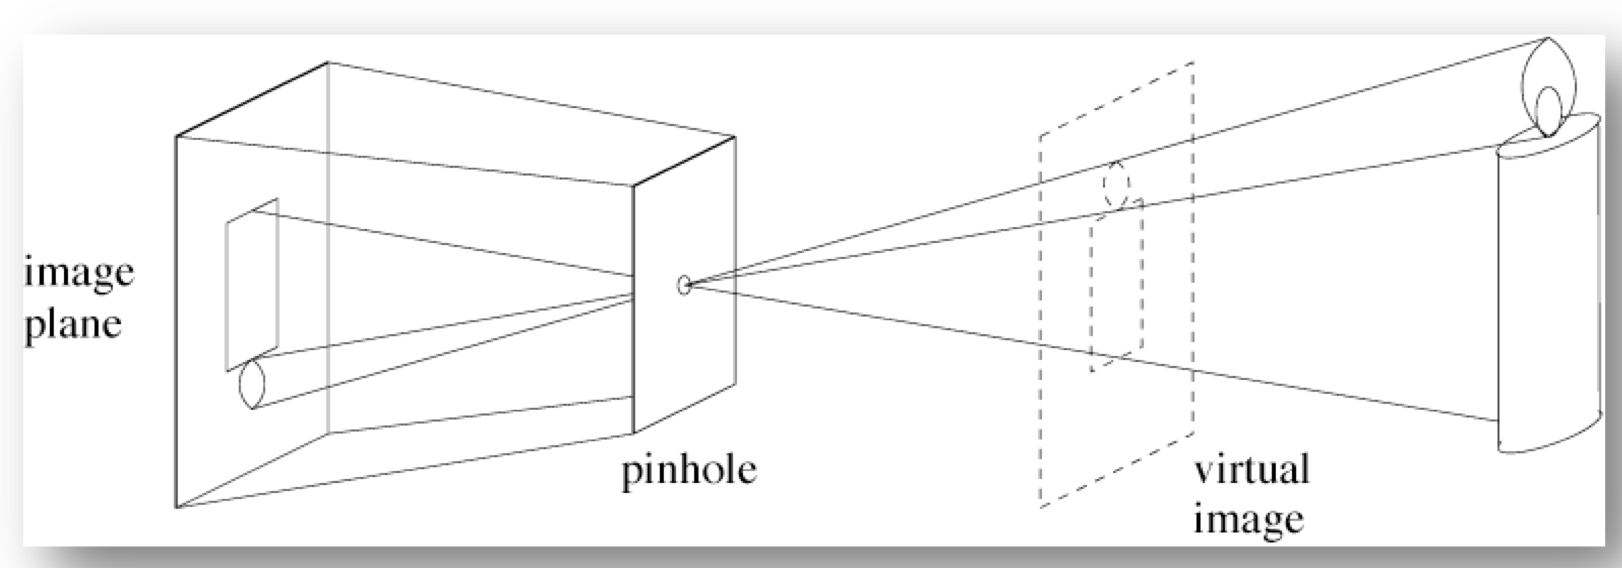
\includegraphics[width=0.5\textwidth]{media/models/pinhole-camera-model.png}
    \caption{Pinhole Camera Model}
\end{figure}
We want to make sure that only a single ray of light from each point passes through the pinhole (ideally, it should be a point), which allows us to create a clear image on the image plane.
Bigger holes would allow multiple rays from the same point to pass through, resulting in a blurry image.

On the image plane, the rays of light from the object are projected, creating an image which is flipped upside down and its size is determined by the distance between the object and the pinhole and the distance
between the pinhole and the image plane (also known as the \textbf{focal length} $f$). The relationship between the object size, the image size, and the distances can be described using similar triangles, as follows:

\begin{minipage}{0.45\textwidth}
    \centering
    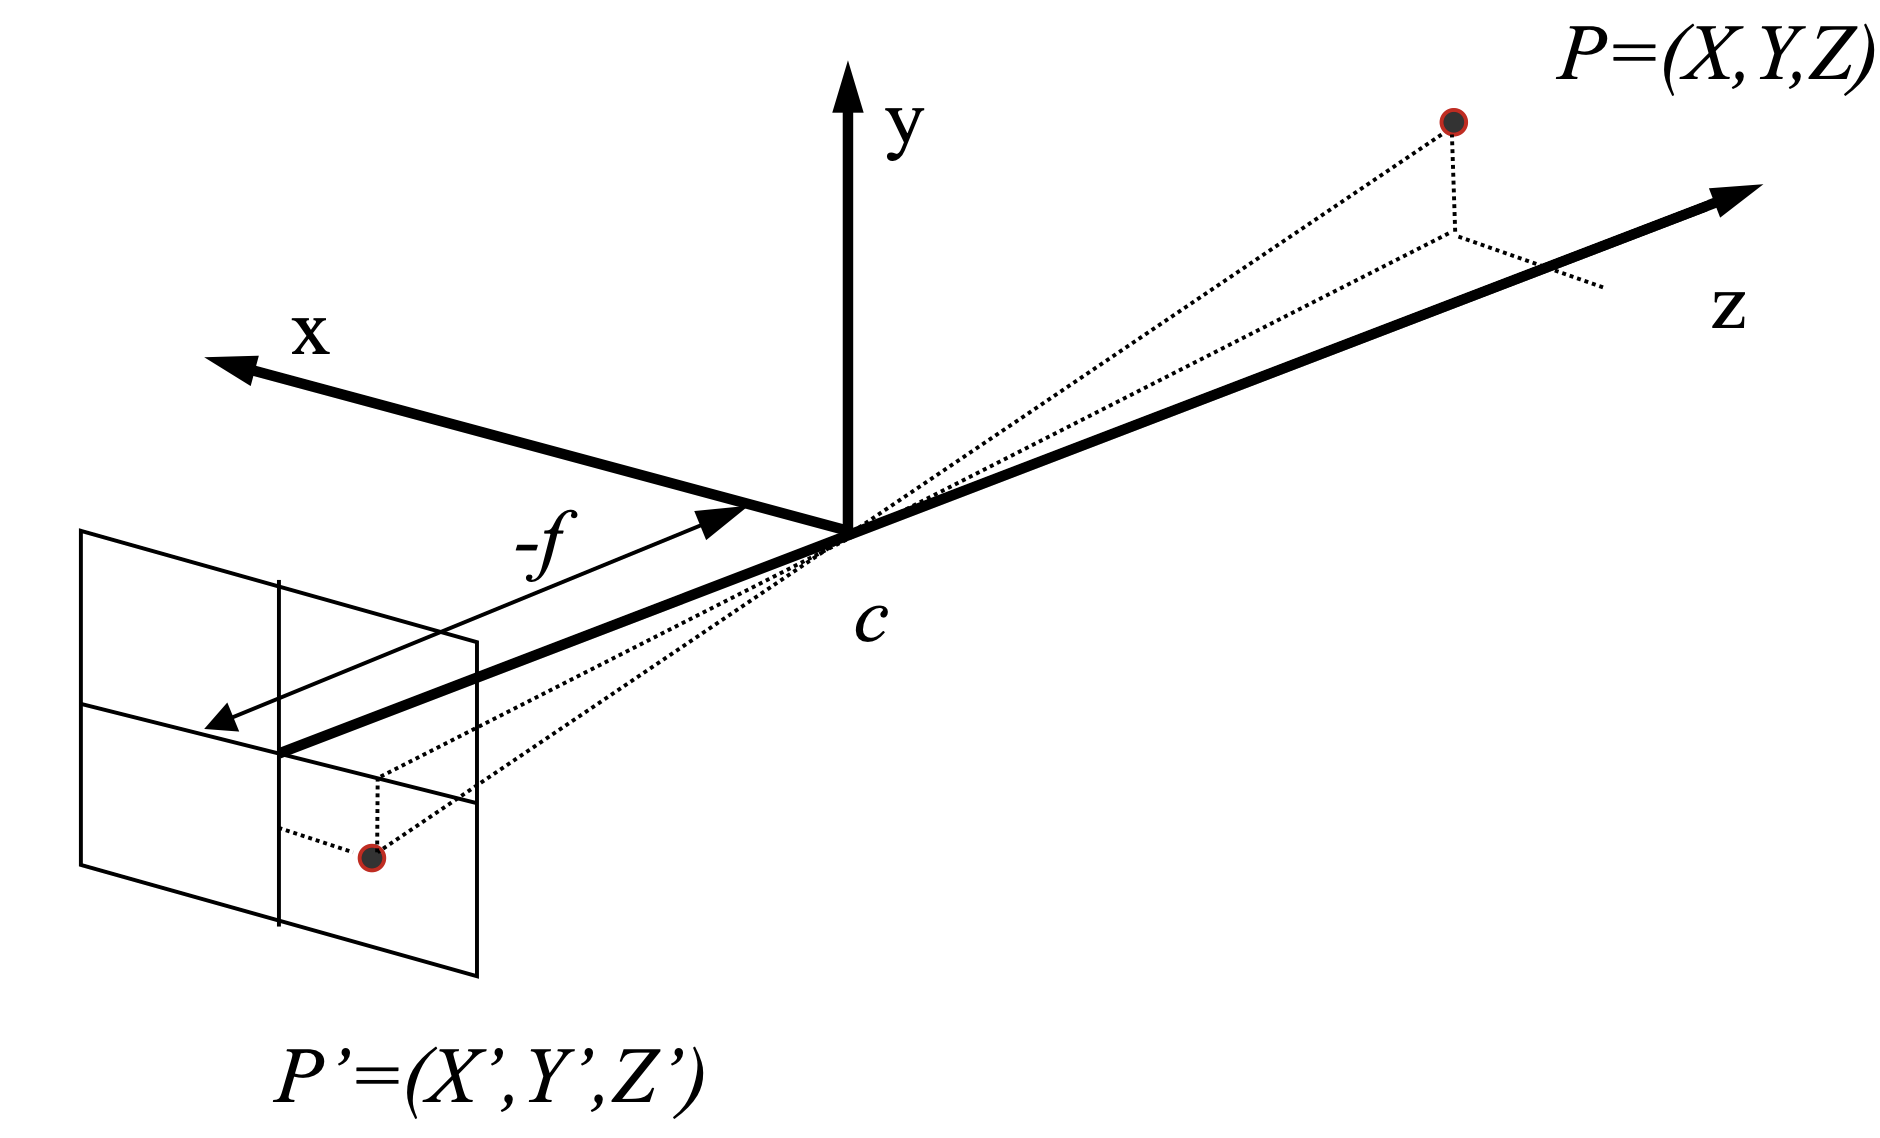
\includegraphics[width=\textwidth]{media/models/projection.png}
    \captionof{figure}{Projection of the point $P$ onto the image plane}
\end{minipage}
\hfill
\begin{minipage}{0.45\textwidth}
    \centering
    \scalebox{0.8}{
        \begin{tikzpicture}
    %Define the z axis
    \draw[->, thick] (-3,0) -- (3,0) node[right] {$z$};
    %Define the y axis
    \draw[->, thick] (0,-2) -- (0,2) node[above] {$y$};

    % Add the point P
    \filldraw[black] (2.5,1) circle (2pt) node[above right] {$P = (X, Y, Z)$};
    % Add the point projection P'
    \filldraw[black] (-1.5,-0.6) circle (2pt) node[below left] {$P' = (X', Y', Z')$};
    % Add the trajectory of the ray from P to P'
    \draw[dotted, thick] (2.5,1) -- (-1.5,-0.6);

    % Add the pinhole at the origin c
    \filldraw[black] (0,0) circle (2pt) node[below right] {$C$};

    % Add the focal length f
    \draw[dotted, thick] (0,0) -- (-2.5,0) node[midway, above] {$-f$};

    %Add the projections of triangles
    \draw[dotted, thick] (2.5,1) -- (2.5,0);
    \draw[dotted, thick] (2.5,0) -- (0,0);
    \draw[dotted, thick] (-1.5,-0.6) -- (-1.5,0);
    \draw[dotted, thick] (-1.5,0) -- (0,0);
\end{tikzpicture}
    }
    \captionof{figure}{Projection of the point $P$ onto the image plane (2D representation)}
\end{minipage}

As shown in the figure, the point $P$ in the real world is projected onto the image plane as $P'$. 
The coordinates of $P'$ can be obtained using the geometric properties of the pinhole camera model. 
In particular, the triangles formed by the points $P$, $C$ (the pinhole), and $P'$ are similar, 
which means that the ratios between the corresponding sides are equal.

This leads to the following relations:
\begin{equation*}
\begin{cases}
Z' = -f \\\\
\dfrac{Z}{Z'} = \dfrac{X}{X'} \\\\
\dfrac{Z}{Z'} = \dfrac{Y}{Y'}
\end{cases}
\end{equation*}

Substituting $Z' = -f$ and rearranging the equations, we obtain
\begin{align*}
X' &= -f \frac{X}{Z} \\
Y' &= -f \frac{Y}{Z}
\end{align*}

Therefore, the projection of the 3D point $P=(X,Y,Z)$ onto the image plane is given by
\[
P' = \left(-f \frac{X}{Z},\; -f \frac{Y}{Z},\; -f\right).
\]

\subsubsection{Features of the model}
The pinhole camera model has several important features:
\begin{itemize}
    \item Further objects appear smaller in the image, which is a consequence of the projection process. It is not able to correctly capture the depth information of the scene;
    \item Parallel lines in the real world appear to converge towards a single point in the image, known as the \textbf{vanishing point}. The line connecting the vanishing is called the \textbf{horizon line}.
    Vertical lines in the real world will still appear vertical in the image, being perpendicular to the horizon line;
    \item The image is inverted (upside down) due to the way light rays pass through the pinhole;
    \item The model assumes that the pinhole is infinitely small, which is obviously an idealization. This would also require an infinite
    amount of light to pass through, which is not practical. 
\end{itemize}

\subsection{Projection}
By the time we capture an image, we have already projected the 3D world onto a 2D plane (the image plane).
Considering also the time dimension, we can formalize the projection process as a mapping from a 4D space to a 3D space:
\[f: \mathbb{R}^4 \rightarrow \mathbb{R}^3\]
\[ (X, Y, Z, t) \mapsto (x, y, t)\]

We can represent two types of projections: \textbf{perspective projection} and \textbf{orthographic projection}.

\subsubsection{Perspective Projection}
Similar to the pinhole camera model, the perspective projection captures the way objects appear smaller as they are further away from the camera.
The only difference is that now the image plane is placed on the origin of the coordinate system, while the pinhole (lens center) is placed between the image plane and the object,
at a distance equal to the focal length $f$.
\begin{figure}[H]
    \centering
    \scalebox{0.8}{
        \input{Tikz/models/perspective-projection-2d.tex}
    }
    \caption{Perspective Projection}
\end{figure}
The triangles formed by the points $P$, $C$ (the pinhole), and $P'$ are again similar, which leads to the following relations:
\begin{equation*}
\begin{cases}
Z' = 0 \\\\
\dfrac{f}{Z - f} = \dfrac{x}{X} \\\\
\dfrac{f}{Z - f} = \dfrac{y}{Y}
\end{cases}
\end{equation*}

Substituting $Z' = 0$ and rearranging the equations, we obtain
\begin{align*}
x &= f \frac{X}{Z - f} \\
y &= f \frac{Y}{Z - f}
\end{align*}

Therefore, the projection of the 3D point $P=(X,Y,Z)$ onto the image plane is given by
\[
P' = \left(f \frac{X}{Z - f},\; f \frac{Y}{Z - f},\; 0\right).
\]
We can notice that knowing the coordinates of the projection $P'$ and the focal length $f$, we cannot recover the original coordinates of the point $P$, since we have two equations and three unknowns.
This is a consequence of the fact that we have lost the depth information during the projection process, which is a fundamental limitation of the perspective projection model.
In case two cameras are used to capture the same scene from different viewpoints, we can use the information from both images to recover the depth information of the scene.

\subsubsection{Simplified Perspective Projection}
The previous model still suffer from the limitation of the pinhole camera model, that flips the image upside down. 
We can easily fix this by placing a virtual image plane between the pinhole and the object, at a distance equal to the focal length $f$.
\begin{figure}[H]
    \centering
    \scalebox{0.8}{
        \begin{tikzpicture}
    %Define the z axis
    \draw[->, thick] (-3,0) -- (3,0) node[right] {$z$};
    %Define the y axis
    \draw[->, thick] (0,-2) -- (0,2) node[above] {$y$};

    % Add the point P
    \filldraw[black] (2.5,1) circle (2pt) node[above right] {$P = (X, Y, Z)$};
    % Add the point projection P'
    \filldraw[black] (1.5,0.6) circle (2pt) node[above left] {$P' = (x, y, z)$};
    % Add the trajectory of the ray from P to C
    \draw[dotted, thick] (2.5,1) -- (0,0);

    % Add the pinhole at the origin c
    \filldraw[black] (0,0) circle (2pt) node[below right] {$C$};

    % Add the focal length f
    \filldraw[black] (1.5,0) circle (2pt) node[below] {$f$};

    %Add the projections of triangles
    \draw[dotted, thick] (2.5,1) -- (2.5,0);
    \draw[dotted, thick] (2.5,0) -- (0,0);
    \draw[dotted, thick] (1.5,0.6) -- (1.5,0);
\end{tikzpicture}
    }
    \caption{Simplified Perspective Projection.}
\end{figure}
The final equations for the projection of the 3D point $P=(X,Y,Z)$ onto the image plane are the same as in the perspective projection model, removing the term $-f$ from the denominator:
\[P' = \left(f \frac{X}{Z},\; f \frac{Y}{Z},\; 0\right).\]
It's important to note that this model is a simplification of the perspective projection model, which is only valid when $f \ll Z$, meaning that the focal length is much smaller than the distance between the object and the camera.
In the real world, this is often the case, since the focal length of a camera is typically a few millimeters, while the distance between the camera and the objects in the scene is usually much larger.

\subsubsection{Orthographic Projection}
In the orthographic projection, we assume that all the rays of light from the object are parallel to each other and perpendicular to the image plane.
This means that the size of the object in the image does not change with distance, and there is no perspective distortion.
\begin{figure}[H]
    \centering
        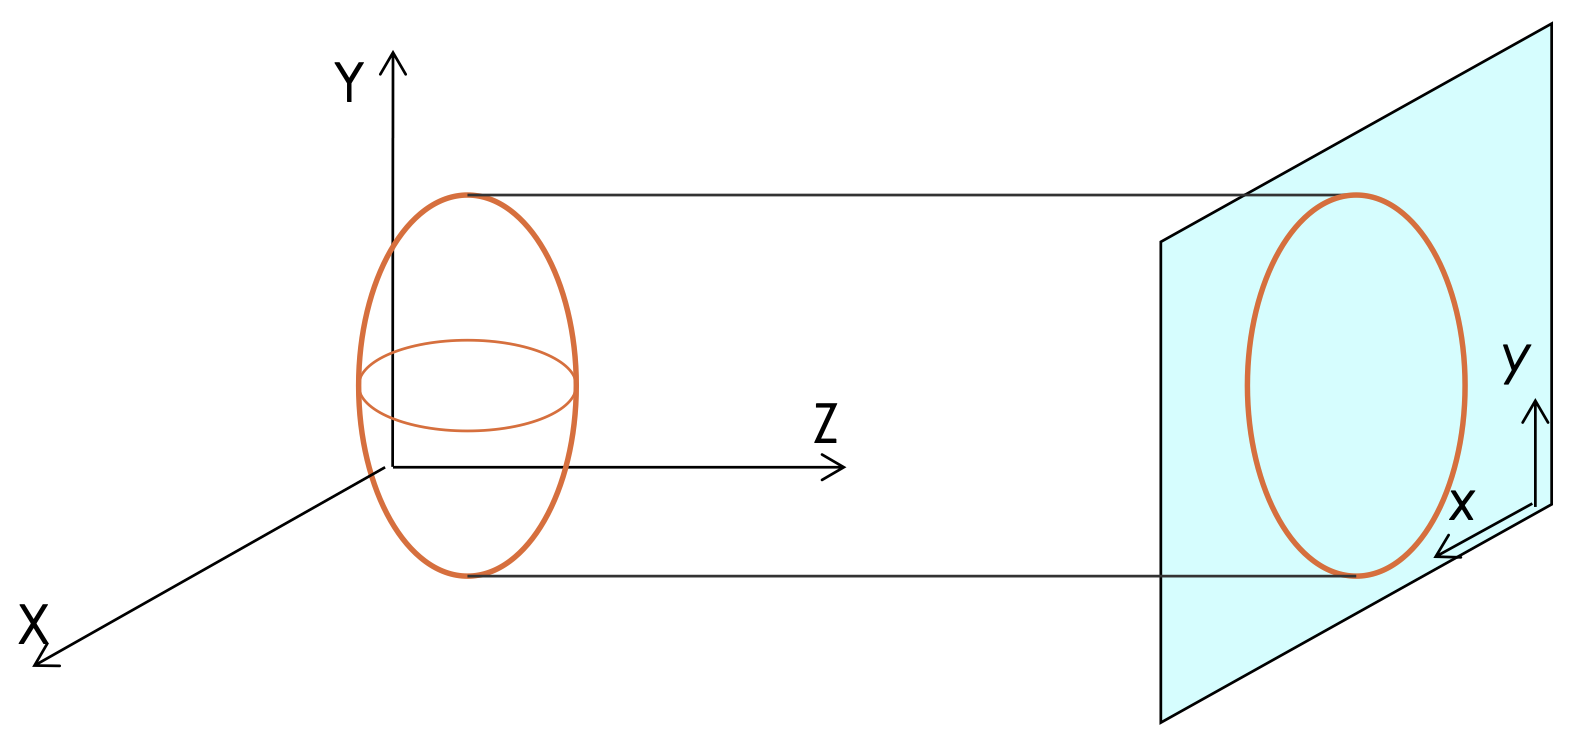
\includegraphics[width=0.5\textwidth]{media/models/orthographic-projection.png}
        \caption{Orthographic Projection model.}
\end{figure}
This assumption is valid when the distance between the camera and the objects in the scene is much larger than the depth of the scene, which is often the case in applications such as satellite imaging or architectural drawings.

The projection of a 3D point $P=(X,Y,Z)$ onto the image plane in the orthographic projection model is given by
\[P' = (X, Y, 0)\] This could also be rewritten in matrix form as follows:
\[
    \begin{bmatrix} x \\ y \end{bmatrix} = \begin{bmatrix} 1 & 0 & 0 \\ 0 & 1 & 0 \end{bmatrix} \begin{bmatrix} X \\ Y \\ Z \end{bmatrix}
\]
We can see this as a special case of the perspective projection model, where the focal length $f$ is infinite, which means that the rays of light are parallel to each other and perpendicular to the image plane.

\subsection{Illumination Model}
Illumination plays a very critical role in Computer Vision. 
The way light interacts with objects in the scene can significantly affect the appearance of the objects in the image, and thus, the performance of computer vision algorithms.

When a light source hits an object, it can be \textbf{absorbed}, \textbf{reflected}, or \textbf{transmitted} through the object.

This is quite difficult to model from the camera's perspective, since we perceive objects based on the light that is reflected from them.

\subsubsection{Reflection}
Reflection can be of two types:
\begin{itemize}
    \item \textbf{Specular}: more energy is concentrated in the light source direction;
    \item \textbf{Diffuse}: constant energy in all directions. The position of the observer is irrelevant,
\end{itemize}

\subsubsection{Surface Properties}
The type of reflection depends on the surface properties of the object, such as its roughness, color, and texture.
Some of them reflect light uniformly in all directions (matte surfaces), while others reflect light in a more concentrated manner (glossy surfaces).

It would be ideal if all objects had matte surfaces, since they would be easier to model and analyze, while glossy surfaces can create artifacts in the image, which can make it difficult to extract useful information from the image.

\subsubsection*{Lambertian Surfaces}
Let's first suppose that we have only one light source which is far away from the scene, so that we can assume that all the rays of light emitted from the light source are parallel to each other.

For each surface point the light is irradiated considering the cosine of the angle between the \textbf{surface normal} and the \textbf{light direction}, which is known as the \textbf{Lambert's cosine law}.
This means that the intensity of the light reflected from a surface point is proportional to the \textbf{cosine} of the \textbf{angle} between the surface normal and the light direction.
Letting $i$ be the intensity of the reflected light, $s$ be the intensity of the light source, $n$ be the surface normal, we can write the Lambert's cosine law as follows:
\[i = s \cdot n\]
This approximation is valid only for \textbf{diffuse reflection}, where the surface reflects light uniformly in all directions.
This is not a realistic model for all surfaces, but it still provides a useful approximation which can be turned into a parametric model.

\subsubsection*{Lambertian Reflectance Model}
The Lambertian reflectance model is a simple model that describes the way light is reflected from a surface point, assuming that the surface is a Lambertian surface.
The model can be expressed as follows:
\begin{equation}
    \label{eq:lambertian_reflectance_model}
    i = \rho s \cdot n \cdot
\end{equation}
which can be computed as:
\[ i = \rho \|n\| \|s\| \cos(\alpha)\]
where $\rho$ is the albedo of the surface, which represents the fraction of light that is reflected from the surface, and $l$ is the light direction.